\section{Le boost de gradient}
\label{chap4.section4}
Le boost de gradient est un autre algorithme d'ensemble mais appartenant à une autre famille d'ensemble que la forêt aléatoire: les boosteurs (\textbf{Boosting ensemble}). Le point commun reste la philosophie des ensembles\footnote{Vulgairement dit, la philosophie des ensembles se base sur l'idée que en associant des apprenants faibles possédant divers bias et faiblesses on peut obtenir un modèle une approximation plus précise de la fonction qui génère les données} mais la méthode est différente.

En effet, là où les techniques de bagging comme la forêt aléatoire combine les prédictions de plusieurs apprenant faibles sur-ajustés pour avoir un modèle plus robuste et des prédictions corrigées par les divers bias des uns et des autres; les techniques de boosting s'appuie sur la \textbf{superposition} de plusieurs apprenants faibles \textbf{sous-ajustés}\footnote{Le sous-ajustement est l'inverse du sur-ajustement et se dit d'un modèle qui échoue à cerner les relations entre les variable indépendantes et la variable dépendante résultant en un modèle très instable.}, généralement aussi des arbres de décision, pour améliorer les performances globales de l'ensemble. L’idée de base est que chaque arbre tente de prédire et donc de corriger les erreurs de tous ses prédécesseurs (\cite{friedman2001greedy}). 

\subsection{Algorithme}
\label{chap4.sec4.sub1}
L’algorithme général est le suivant:

\begin{enumerate}
    \item \textbf{Initialisation}: Initialiser le « réseau », avec un apprenant très faibles, généralement une constante comme la moyenne des étiquettes de l'ensemble d'entraînement ou les chances logarithmiques de chaque classe selon si le problème d'apprentissage est un problème de régression ou de classification.
    \begin{itemize}
        \item \textbf{Régression}: Initialiser avec la moyenne des étiquettes (labels) de l'ensemble d'entraînement \[\hat{y}^{(0)} = mean(y)\]
        \item \textbf{Classification}: Initialiser avec un modèle qui retourne la probabilité logarithmique\footnote{La chance logarithmique d'une probabilité est le logarithme népérien de la probabilité que cet événement se produise. Il transforme une valeur de probabilité \(p\) allant de 0 à 1 en une valeur réelle allant de \(-\infty\) à \(+\infty\).} des différentes classes. \[\hat{y}^{(0)} = logit(y) = log(\frac{p}{1 - p})\] où \(p\) est la probabilité de la classe positive dans l'ensemble d'entraînement si le problème est une classification binaire ou le vecteur des probabilités de chaque classe sinon.
    \end{itemize}
    \item \textbf{Iteration}: Calculez ensuite l'erreur résiduelle de ces premières prédictions pour entraîner un arbre avec celle-ci comme target. À part des changement arbitraire pour le critère de sélection de l'attribut le plus important, l'algorithme reste le même que celui décrit dans la section \ref{chap4.sec2.sub3}. Après l'arbre entraîné est ajouté à l'ensemble avec un taux d'apprentissage\footnote{Le taux d'apprentissage est un nombre réel relativement petit utilisé comme une sorte de poids pour contrôler la vitesse d'apprentissage de l'ensemble. En gros il est là pour que la contribution d'un arbre à l'ensemble ne soit pas trop grand par rapport aux autres} en le superposant aux arbres précédents où il servira à prédire l'erreur de ces derniers. Cette étape est répétée jusqu'à ce que nous atteignions un certain nombre d'arbres ou d'itération. Le processus d'ajout séquentiel d'un nouvel arbre pour prédire l'erreur du précédent est analogue à la descente de gradient dont on parlera dans la prochaine section, d'où le nom boost de \textbf{gradient}. Formellement ça donne:

    Pour \(m\) de 1 à \(M\) (nombre d'iteration/arbre)
    \begin{itemize}
        \item \textbf{Calculez les erreurs résiduelle}: L'erreur résiduelle est la différence entre les vraies étiquettes et les prédictions de l'ensemble\[r_i^{(m)} = y_i - \hat{y}_i^{(m-1)}\]
        \item \textbf{Entraîner un arbre de régression}: Entraîner un arbre de régression avec les données de l'ensemble d'entraînement comme entrées et les erreurs résiduelles comme sortie. Le but de cet arbre est de prédire l'erreur de l'ensemble, raison pour laquelle tous les arbres intermédiaires sont des arbres de régression.
        \item Ajoutez les prédictions du nouvel arbre pondérés par le taux d'apprentissage aux prédictions de l'ensemble actuel. \[\hat{y}_i^{(m)} = \hat{y}_i^{(m-1)} + \eta \cdot h_m(x_i)\] où \(h_m(x_i)\) est la prédiction du nouvel arbre pour l'erreur de l'ensemble sur l'exemple \(i\) de l'ensemble d'entraînement.
    \end{itemize}
    
    \item \textbf{Prédiction final}: Enfin, le modèle fait une prédiction pour chaque \(x_i\) de l'ensemble de test en ajoutant les prédictions de tous les arbres (pondérées par le taux d'apprentissage). Pour un problème de classification, ce résultat est transmis à une fonction de seuillage ou de convertion en probabilité.
    \begin{itemize}
        \item \textbf{Pour la régression}: \[\hat{y}_i^{final} = \hat{y}^{(0)} + \Sigma_{m=1}^M \eta \cdot h_m(x_i)\]
        \item \textbf{Pour la classification}: il suffit de reconvertir \(\hat{y}_i^{final}\) qui sera sera alors la chance logarithmique des différentes classes grâce à une fonction comme celle ci (soyez attentif à cette fonction, on la reverra plus tard): \[p_i^{final} = \frac{1}{1 + e^{-\hat{y}_i^{final}}}\]
    \end{itemize}
\end{enumerate}

Une illustration de l'algorithme est montré dans la figure \ref{fig:fig6}

\begin{figure}
    \centering
    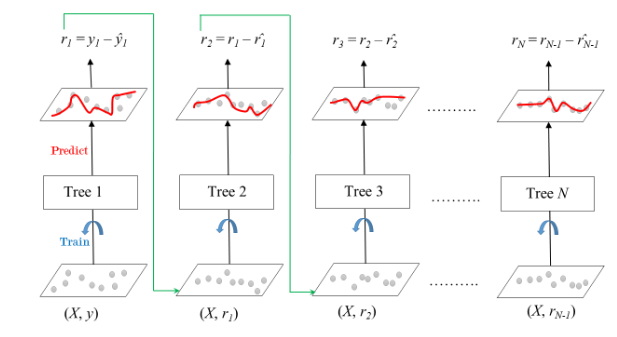
\includegraphics[width=0.75\linewidth]{images/gradientboosting.png}
    \caption{Illustration de l'algorithme de boost de gradient (\cite{geeksforgeeks2023gradient})}
    \label{fig:fig6}
\end{figure}

\subsection{Implémentation}
\label{chap4.sec4.sub2}
Le plus gros inconvénient des modèles non paramètriques en général est que le temps nécéssaire pour leur entraînement augmente avec la taille de l'ensemble d'entraînement et les techniques de boosting sont particulièrement démonstratifs de cette faille. Donc on utilise souvent des versions un peu modifiées, voir tronquées, de l'algorithme ci-dessus quand on a à faire à de grands ensembles de données (\cite{odegua2020predicting}). Pour ce projet j'ai donc utilisé l'implémentation de scikit-learn basée sur les histogrammes qui est plus efficace grâce à deux particularités majeures:

\begin{itemize}
    \item \textbf{Discrétisation des valeurs continues}: Les prédicateurs continues sont discrétisées en un nombre fixe de groupes au moment de la construction des arbres de décisions. Vous rappelez vous de l'exemple avec l'âge au début de la section \ref{chap4.section2}? Là où les arbres de décisions classiques utiliseraient chaque valeurs de ces prédicateurs comme branche. Le fait de créer des catégories pour les valeurs continues (catégories qui seront les branches de cet attribut) réduit la précision des valeurs des attributs mais permet un calcul beaucoup plus rapide.
    \item \textbf{Créer des histogrammes}: Pour chaque prédicateur, un histogramme\footnote{Un histogramme est un graphique qui montre la fréquence des données numériques à l'aide de rectangles. La hauteur d'un rectangle (l'axe vertical) représente la fréquence de distribution d'une variable (le montant ou la fréquence d'apparition de cette variable).} est construit en comptant le nombre d'exemples dans chaque branche, d'où le nom \textbf{Histogram-based Gradient Boosting}. Ces histogrammes sont la représentation qui sera utiliser pour entraîner les arbres au lieu de l'ensemble complet, cela permet de reduire significantivement l'usage mémoire et encore une fois d'accélérer l'entraînement des arbres. 
\end{itemize}

Traditionnellement, le prédicateur le plus important (lors de l'entraînement des arbres) est choisi comme étant celui qui minimise la somme de la somme quadratique des erreurs résiduelles dans chaque branche. Cette somme est définie par la formule: \[RSS = \Sigma_{n=1}^M Q_n\] où \(Q_n\) est la somme quadradique des erreurs résiduelles dans la \(n\)ième branche définie par: \[Q_n = \Sigma_i r_i^2\] où \(r_i\) est l'erreur résiduelle du \(i\)ème exemple de la branche. En pratique, pour les problèmes de classifications les erreurs résiduelles sont souvent remplacées par les gradients d'une \textbf{fonction de coût} et le but est de minimiser cette dernière, on détaillera cette approche dans la prochaine section.

Tout comme l'implémentation de la forêt aléatoire mon implémentation du boost de gradient possède 200 arbres, le taux d'apprentissage est fixé à 0,1 et le nombre maximal de groupes lors de la discrétisation des valeurs continues est fixé à 255; notez que cette limite est aussi applicable aux prédicateurs de nature catégorique possédant plus de 255 valeurs uniques(\cite{diarra2024gradient}).